\section{Rezultati eksperimenata}
\label{sec:rezultati-eksperimenata}

Za sva tri eksperimenta opisana u poglavlju~\ref{ch:eksperimenti} prikazani su podaci snimljeni tijekom stvarnog leta (\emph{rosbag} zapis svih tema upravljačkog sloja), ograničeni na razdoblje u kojem je regulator poravnanja stvarno aktivan, od ulaska u stanje \texttt{ALIGN} do njegovog konačnog napuštanja. Svi kutovi na grafovima izraženi su u stupnjevima radi čitljivosti, iako ih upravljački sloj interno računa i objavljuje u radijanima.

\subsection{Eksperiment 1: slijetanje na ArUco oznaku (kamera prema dolje)}
\label{subsec:rez-eksperiment1}

Letjelica je iz stanja \texttt{ALIGN} krenula s pikselnom pogreškom od približno $(25, 40)$ piksela i regulator ju je unutar nešto manje od četiri sekunde sveo na vrijednost unutar praga poravnanja (Slika~\ref{fig:exp1-error}), nakon čega je sustav ušao u stanje \texttt{ALIGNED} i letjelica sletjela. Budući da je upravljački sloj u ovom letu radio u načinu \emph{attitude} (Odjeljak~\ref{subsec:pid-kaskada}), naredba se šalje kao ciljni nagib, a ne kutna brzina, pa je naređeni i stvarni nagib letjelice izravno usporediv na istom grafu. Oba usko prate jedan drugoga tijekom čitavog manevra (Slika~\ref{fig:exp1-angles}), uz zaostajanje AHRS procjene od otprilike 0.2 do 0.3 sekunde iza naredbe, posljedica dinamike letjelice i unutarnje petlje koju zatvara sam ArduPilot. Naredba okomitog kretanja (Slika~\ref{fig:exp1-thrust}) prelazi s vrijednosti mirovanja (0.5) na vrijednost spuštanja (\texttt{land\_descend\_thrust}, 0.45) čim je letjelica bočno unutar praga za spuštanje, i vraća se na mirovanje kad taj prag napusti, potvrđujući opisanu funkcionalnu ovisnost okomitog kretanja o bočnom poravnanju (Odjeljak~\ref{subsec:prijanjanje}).

\begin{figure}[h]
  \centering
  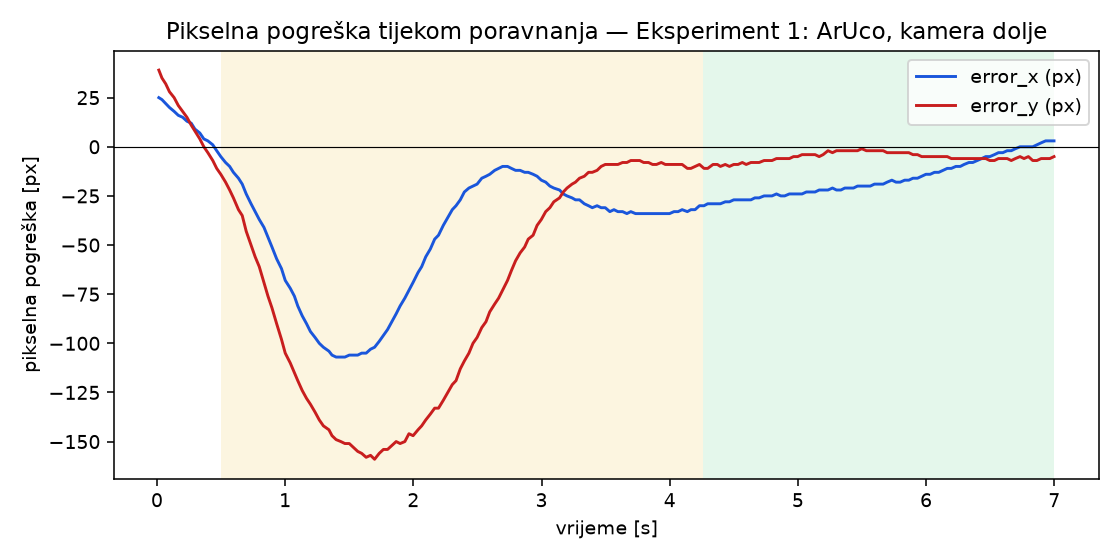
\includegraphics[width=0.85\textwidth]{images/rezultati/exp1_error.png}
  \caption{Pikselna pogreška tijekom prvog eksperimenta. Žuto osjenčano područje označava stanje \texttt{ALIGN}, zeleno stanje \texttt{ALIGNED}.}
  \label{fig:exp1-error}
\end{figure}

\begin{figure}[h]
  \centering
  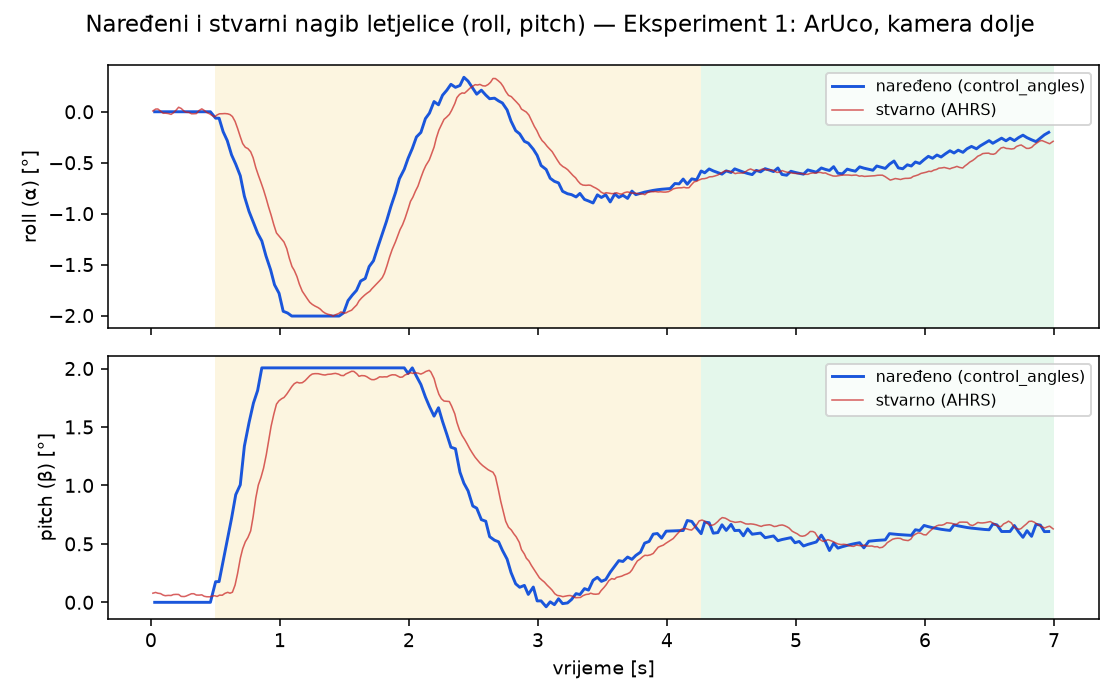
\includegraphics[width=0.85\textwidth]{images/rezultati/exp1_angles.png}
  \caption{Naređeni nagib (izlaz vanjske petlje, nakon ograničenja) i stvarni nagib očitan iz AHRS-a tijekom prvog eksperimenta.}
  \label{fig:exp1-angles}
\end{figure}

\begin{figure}[h]
  \centering
  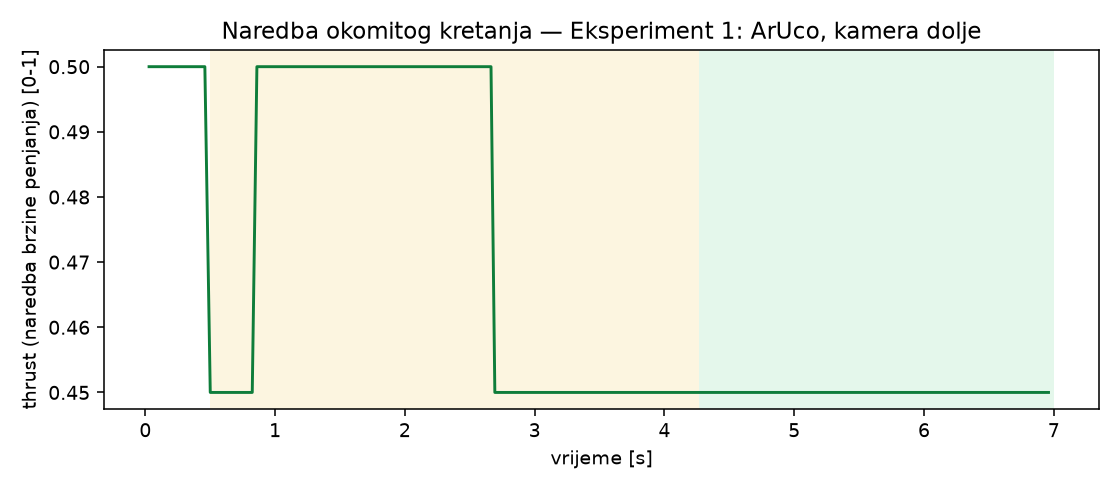
\includegraphics[width=0.85\textwidth]{images/rezultati/exp1_thrust.png}
  \caption{Naredba okomitog kretanja tijekom prvog eksperimenta. Vrijednost 0.5 odgovara mirovanju, niža vrijednost spuštanju.}
  \label{fig:exp1-thrust}
\end{figure}

\subsection{Eksperiment 2: praćenje ArUco oznake (kamera prema gore)}
\label{subsec:rez-eksperiment2}

Nakon preslikavanja osi opisanog u Odjeljku~\ref{subsec:preslikavanje-osi}, letjelica je uspješno poravnala kameru okrenutu prema gore s ArUco oznakom te dosegnula stanje \texttt{ALIGNED}, potvrđujući da preslikavanje osi ispravno funkcionira nakon rotacije kamere za 180 stupnjeva. Nakon ulaska u stanje \texttt{ALIGNED}, pikselna pogreška u ovom konkretnom zapisu nastavlja rasti (Slika~\ref{fig:exp2-error}) sve do povratka u stanje \texttt{ALIGN}, na razini histereznog praga. Ovo ponašanje razmatra se u Odjeljku~\ref{subsec:rasprava-uzdignuti-cilj}. Uz ovu konfiguraciju kamere i istu ArUco detekciju, u zasebnom pokušaju snimljenom na videu letjelica je uspješno izvela i cijeli manevar prijanjanja.

\begin{figure}[h]
  \centering
  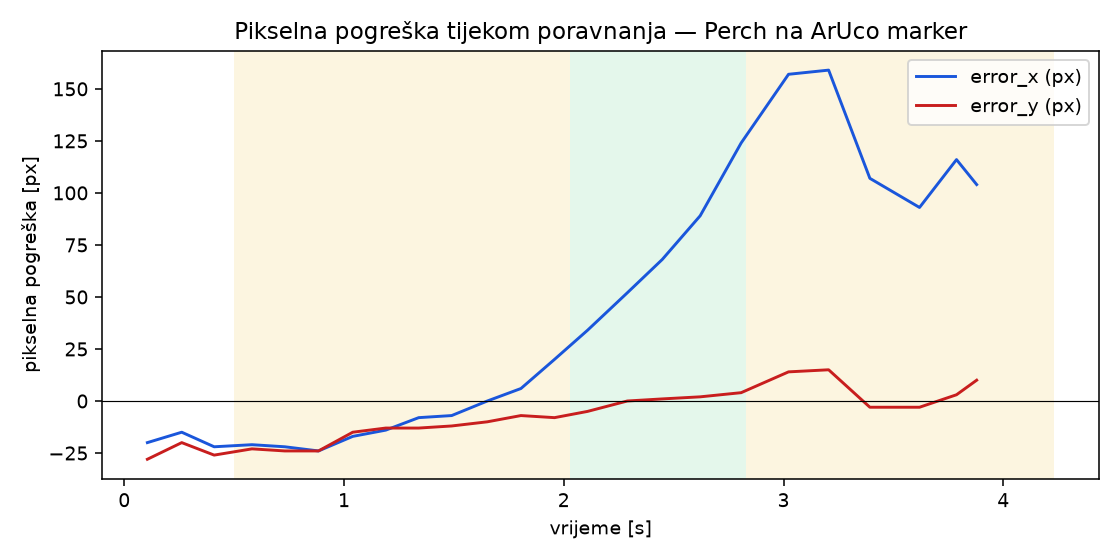
\includegraphics[width=0.85\textwidth]{images/rezultati/exp2_error.png}
  \caption{Pikselna pogreška tijekom drugog eksperimenta. Zeleno osjenčano područje označava stanje \texttt{ALIGNED}.}
  \label{fig:exp2-error}
\end{figure}

\subsection{Eksperiment 3: prijanjanje na granu}
\label{subsec:rez-eksperiment3}

Treći eksperiment rezultirao je uspješnim prijanjanjem na golu granu, bez oznake, korištenjem cjevovoda za detekciju opisanog u poglavlju~\ref{ch:percepcija}. Snimka pokušaja dostupna je kao video prilog radu.

Za uspješni pokušaj, pikselna pogreška (Slika~\ref{fig:exp3-error}) opada iz početne vrijednosti od približno $(-110, -80)$ piksela do nule unutar otprilike 2.7 sekunde, nakon čega slijedi nagli porast pogreške u posljednjoj sekundi prije fizičkog kontakta s granom. Taj porast posljedica je gubitka udaljenosti detekcije od zadanog cilja kako se grana, s približavanjem letjelice, širi preko sve većeg dijela slike i izlazi iz vidnog polja kamere, geometrijski neizbježno u završnoj fazi prijanjanja s kamerom okrenutom prema gore. Letjelica pritom ostaje u stanju \texttt{ALIGN} kroz čitav manevar, sve do naoružavanja isključenog na samom kraju zapisa, nakon fizičkog kontakta s granom. Putanja ciljne točke u slici (Slika~\ref{fig:exp3-target}) potvrđuje tumačenje porasta pogreške: točka se pomiče dijagonalno od gornjeg lijevog dijela slike prema donjem desnom rubu, u skladu sa smjerom u kojem je grana pozicionirana u odnosu na početni položaj letjelice.

Naređeni i stvarni nagib letjelice (Slika~\ref{fig:exp3-rollpitch}) usko prate jedan drugoga do posljednje sekunde prije kontakta, kada dolazi do naglog prekida poravnanja vidljivog u oba grafa kao posljedica gubitka detekcije uslijed kontakta i mehaničkog trzaja pri hvatanju.

\begin{figure}[h]
  \centering
  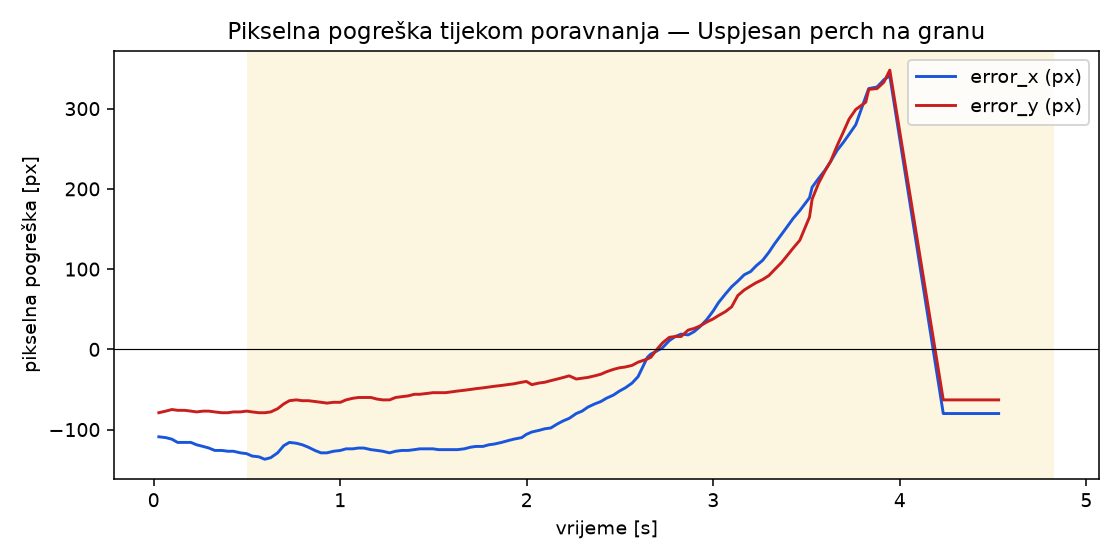
\includegraphics[width=0.85\textwidth]{images/rezultati/exp3_error.png}
  \caption{Pikselna pogreška tijekom uspješnog prijanjanja na granu.}
  \label{fig:exp3-error}
\end{figure}

\begin{figure}[h]
  \centering
  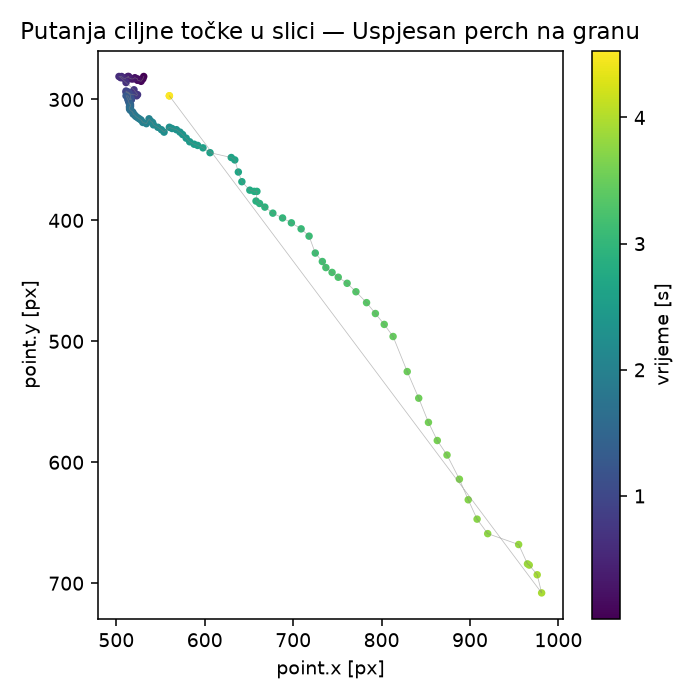
\includegraphics[width=0.6\textwidth]{images/rezultati/exp3_target_traj.png}
  \caption{Putanja ciljne točke u slikovnoj ravnini tijekom uspješnog prijanjanja na granu, obojena prema vremenu.}
  \label{fig:exp3-target}
\end{figure}

\begin{figure}[h]
  \centering
  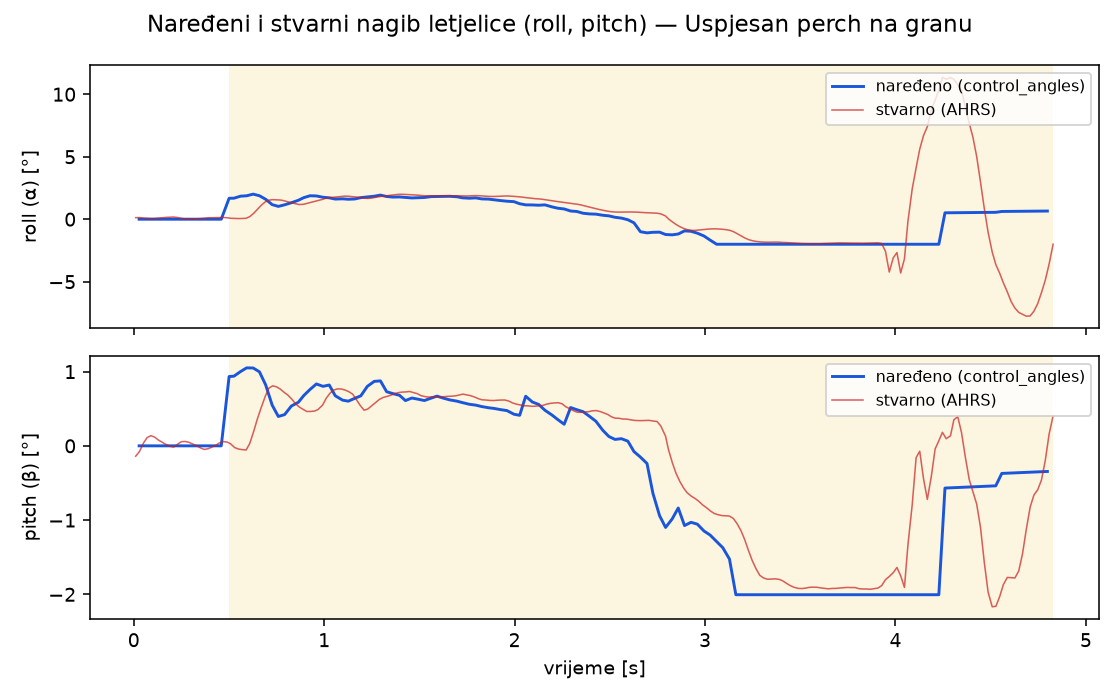
\includegraphics[width=0.85\textwidth]{images/rezultati/exp3_rollpitch.png}
  \caption{Naređeni i stvarni nagib letjelice (roll, pitch) tijekom uspješnog prijanjanja na granu.}
  \label{fig:exp3-rollpitch}
\end{figure}

\begin{figure}[h]
  \centering
  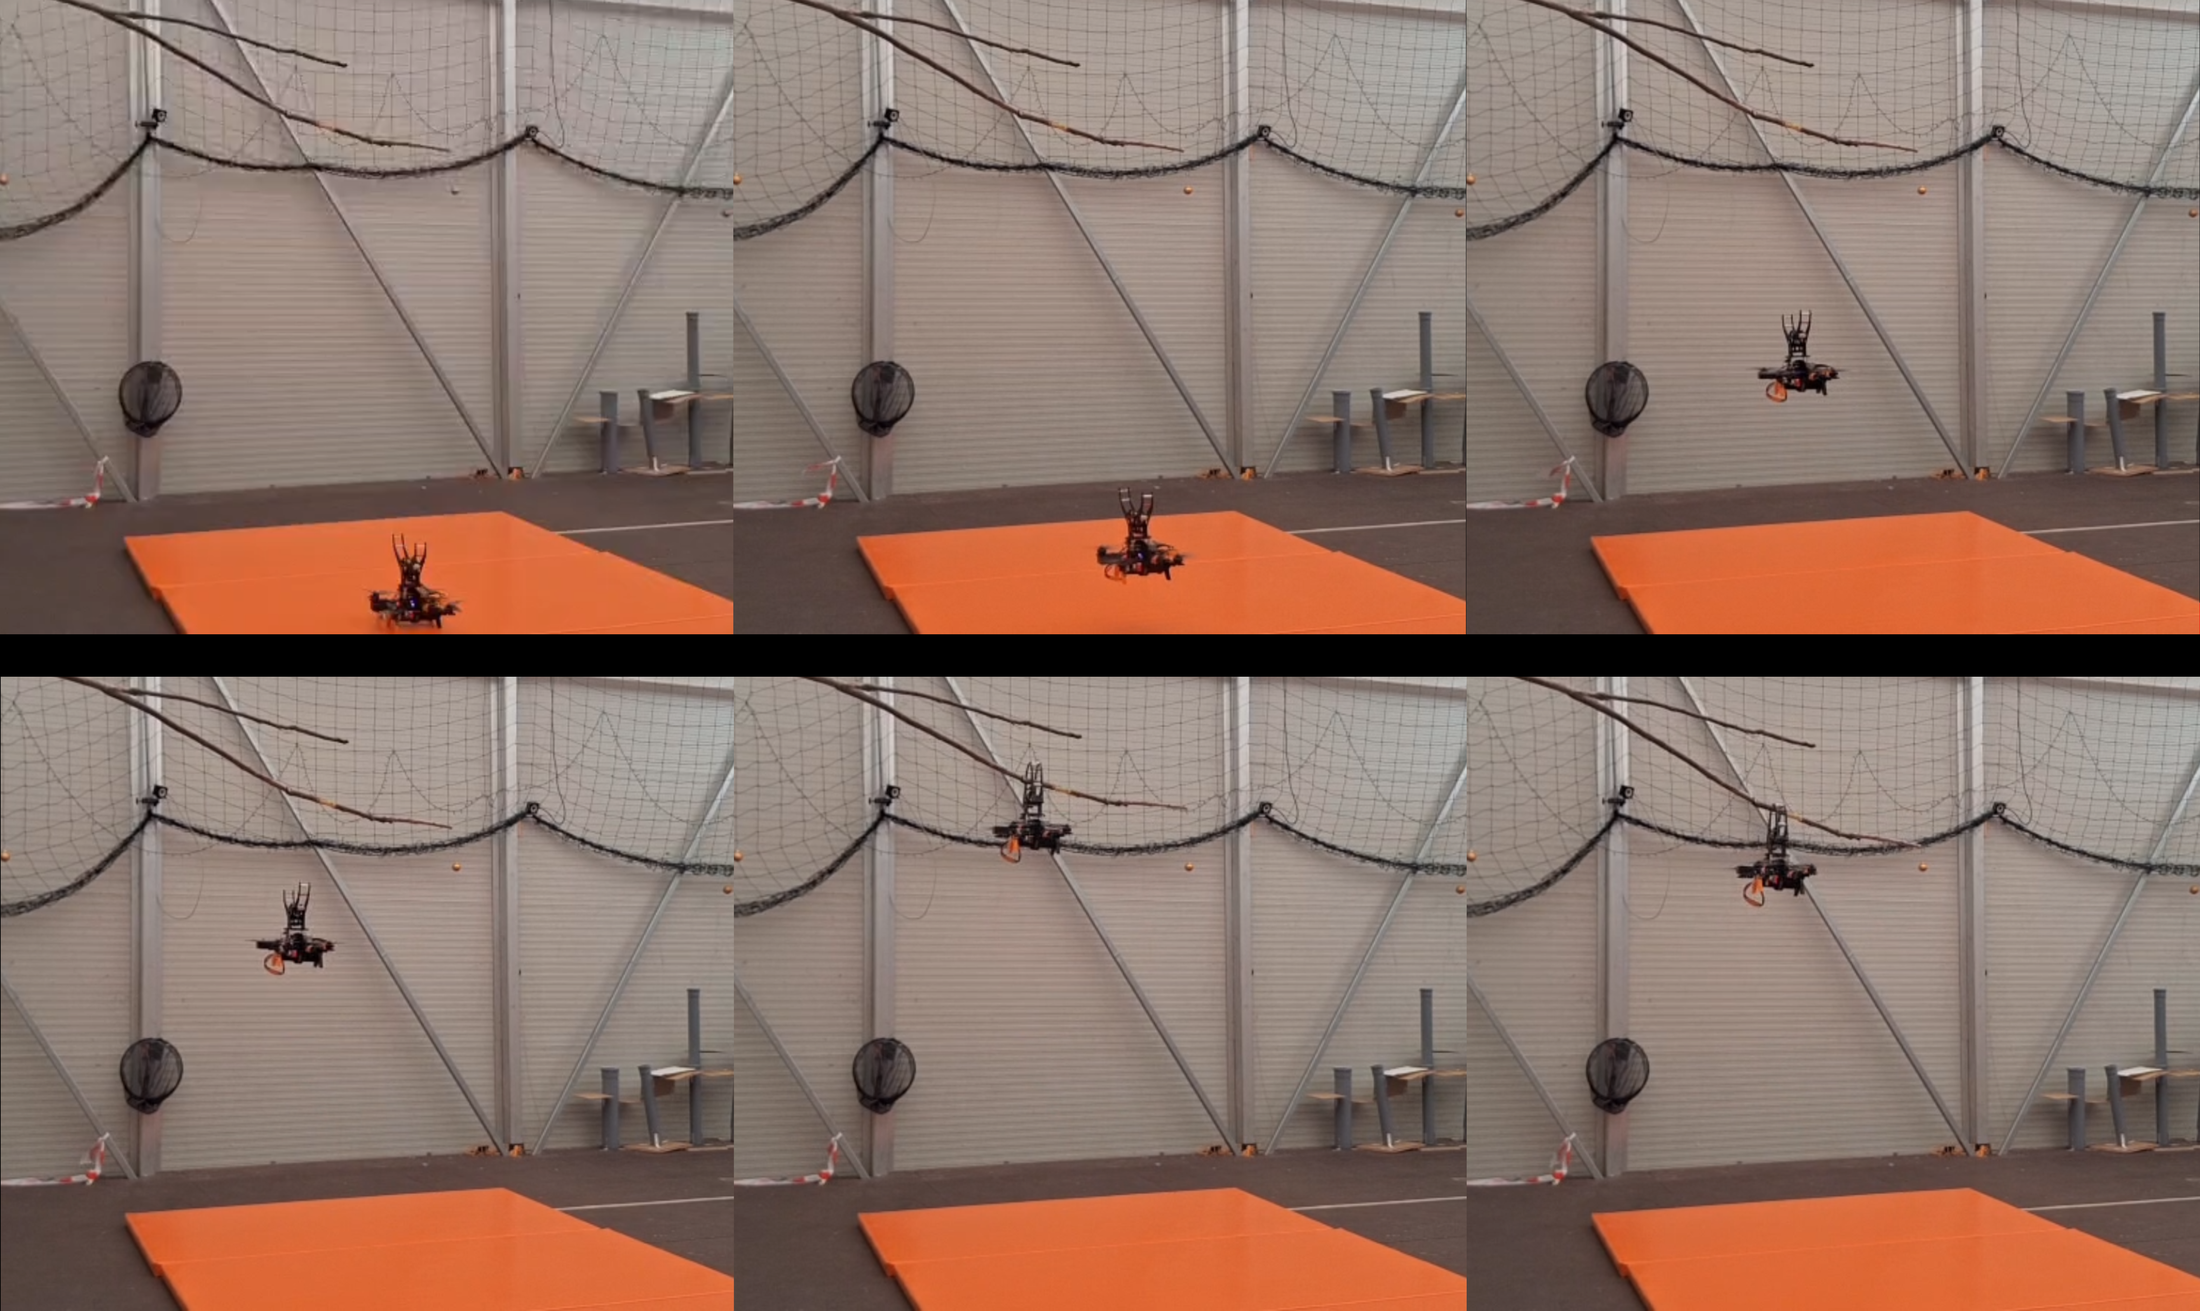
\includegraphics[width=1.0\textwidth]{images/rezultati/exp3_timeline.png}
  \caption{Vremenski slijed uspješnog prijanjanja na granu: uzlijetanje, penjanje, prilazak i hvatanje grane.}
  \label{fig:exp3-success-frame}
\end{figure}

\section{Rasprava}
\label{sec:rasprava}

\subsection{Ostvarenje ciljeva rada}
\label{subsec:rasprava-ciljevi}

Rezultati eksperimenata potvrđuju sva četiri cilja postavljena u Odjeljku~\ref{sec:ciljevi}. Cjevovod za detekciju grane i praćenje točke prijanjanja radi bez ugrađene pretpostavke o orijentaciji kamere, budući da izlaz cjevovoda ostaje jednak pikselnom položaju bez obzira gleda li kamera prema dolje ili prema gore, dok se sva prilagodba geometriji odvija isključivo u preslikavanju osi na upravljačkoj strani (Odjeljak~\ref{subsec:preslikavanje-osi}). Upravljanje letjelicom paketom \texttt{ibvs\_perching} ostvareno je bez vanjske lokalizacije, oslanjajući se isključivo na AHRS procjenu orijentacije i izravno slanje naredbi preko sučelja \texttt{mavros/setpoint\_raw/attitude}, potvrđeno u sva tri eksperimenta. Preslikavanje osi za kameru okrenutu prema gore implementirano je i eksperimentalno potvrđeno drugim i trećim eksperimentom, koji pokazuju da letjelica ispravno poravnava bočni položaj s ciljem iznad sebe. Naposljetku, eksperimentalna provjera provedena je kroz tri opisana koraka rastuće složenosti, pri čemu je treći korak rezultirao uspješnim prijanjanjem na granu bez ijedne oznake ili vanjskog referentnog sustava.

\subsection{Ponašanje nakon dosezanja stanja poravnano}
\label{subsec:rasprava-uzdignuti-cilj}

U drugom eksperimentu (Odjeljak~\ref{subsec:rez-eksperiment2}) pogreška nastavlja rasti i nakon ulaska u stanje \texttt{ALIGNED}, sve do napuštanja tog stanja na histereznom pragu. Ovo je izravna posljedica dizajna praga za spuštanje/penjanje opisanog u Odjeljku~\ref{subsec:prijanjanje}: budući da je taj prag postavljen jednako širokim kao i prag za ulazak u stanje \texttt{ALIGNED}, sustav dopušta rub tolerancije u kojem je letjelica još uvijek unutar dozvoljenog raspona za okomito kretanje, ali izvan raspona koji regulator uspijeva stabilno održavati bez daljnjeg poremećaja. Kod treće provjere, s cjevovodom za detekciju grane, ovo se ponašanje ne očituje na isti način jer manevar prijanjanja završava fizičkim kontaktom s granom prije nego što bi do takvog odstupanja moglo doći.

\subsection{Vezanost pomaka slike i nagiba letjelice}
\label{subsec:rasprava-coupling}

Grafovi pikselne pogreške u sva tri eksperimenta povremeno pokazuju kratkotrajne skokove pogreške usred inače glatkog pada prema nuli. Ovi skokovi nisu posljedica šuma u detekciji, nego izravne fizičke vezanosti (\emph{coupling}) između nagiba letjelice i pomaka slike: kamera je kruto pričvršćena na letjelicu, pa svaki nagib koji regulator naredi radi smanjenja pogreške istovremeno zakreće i sam vidokrug kamere. Taj zakret pomiče cilj u slici u smjeru suprotnom od očekivanog trenutak prije nego što stvarno translacijsko gibanje letjelice počne smanjivati pogrešku, što se u grafu očituje kao kratak, mali porast pogreške upravo u trenutku kada regulator poveća naredbu nagiba. Ova je pojava svojstvena samoj geometriji sustava (kamera kruto vezana za tijelo letjelice bez vlastite stabilizacije nagiba) i ne predstavlja kvar ili nestabilnost regulatora.

\subsection{Održavanje visine pri naredbi mirovanja}
\label{subsec:rasprava-barometar}

Vrijednost naredbe okomitog kretanja 0.5 protumačena je kao naredba mirovanja, odnosno nulte brzine penjanja (Odjeljak~\ref{subsec:prijanjanje}). U idealnim uvjetima to bi značilo da letjelica pri toj naredbi zadržava potpuno nepromijenjenu visinu. U stvarnosti, procjena visine unutar ArduPilota oslanja se na barometarsko mjerenje tlaka, na koje utječe strujanje zraka koje stvaraju vlastiti propeleri letjelice te ograničena preciznost samog barometarskog senzora. Zbog toga naredba mirovanja u praksi ne drži letjelicu na potpuno istoj visini, nego letjelica postupno odstupa dok ArduPilotov regulator visine unutar GUIDED načina rada tu promjenu ne prepozna kao dovoljno značajnu da ju počne aktivno korigirati. Ova nesavršenost održavanja visine dio je razloga za oscilacije vidljive na grafovima naredbe okomitog kretanja, uz vezanost opisanu u Odjeljku~\ref{subsec:rasprava-coupling}.

\subsection{Ograničenje okidanja prijanjanja bez izravnog mjerenja udaljenosti}
\label{subsec:rasprava-okidanje}

Sustav namjerno ne koristi senzor udaljenosti niti bilo kakav diskretni signal za okidanje trenutka prijanjanja (Odjeljak~\ref{subsec:prijanjanje}), nego se penjanje odvija kontinuirano dok je letjelica bočno poravnata, sve dok mehanizam za prijanjanje fizički ne dosegne granu. Ovakav pristup izbjegava ovisnost o dodatnom senzoru, ali prenosi odgovornost za uspješnost hvatanja isključivo na točnost bočnog poravnanja i geometrijski razmak između kamere i hvataljke (Odjeljak~\ref{subsec:test3-postav}). Posljedica je da sustav nema način unaprijed prepoznati da hvatanje neće uspjeti: ako letjelica u trenutku fizičkog kontakta nije dovoljno točno poravnata, manevar se ne zaustavlja niti ponavlja sam od sebe, nego zahtijeva da sigurnosni pilot prekine pokušaj.

\subsection{Utjecaj skupa podataka za treniranje na novu konfiguraciju kamere}
\label{subsec:rasprava-dataset}

Skup podataka za treniranje modela detekcije (Odjeljak~\ref{sec:treniranje-modela}) sniman je pretežno iz bočne perspektive, u skladu s izvornim scenarijem prilaska grani. U scenariju ovog rada, kamera gleda prema gore i grana se u posljednjoj fazi prijanjanja vidi pod znatno oštrijim kutom te bliže rubu ili izvan kadra nego što je slučaj u velikom dijelu skupa za treniranje. Uspješno prijanjanje u trećem eksperimentu pokazuje da model unatoč tome generalizira dovoljno dobro za ovu primjenu, no rastuća pogreška u posljednjoj sekundi prije kontakta (Odjeljak~\ref{subsec:rez-eksperiment3}) dijelom proizlazi i iz ove promjene perspektive, budući da grana pod oštrim kutom zauzima drugačiji oblik u slici nego u većini primjera korištenih za treniranje.

